\documentclass[12pt]{article}\usepackage[]{graphicx}\usepackage[]{color}
%% maxwidth is the original width if it is less than linewidth
%% otherwise use linewidth (to make sure the graphics do not exceed the margin)
\makeatletter
\def\maxwidth{ %
  \ifdim\Gin@nat@width>\linewidth
    \linewidth
  \else
    \Gin@nat@width
  \fi
}
\makeatother

\definecolor{fgcolor}{rgb}{0.345, 0.345, 0.345}
\newcommand{\hlnum}[1]{\textcolor[rgb]{0.686,0.059,0.569}{#1}}%
\newcommand{\hlstr}[1]{\textcolor[rgb]{0.192,0.494,0.8}{#1}}%
\newcommand{\hlcom}[1]{\textcolor[rgb]{0.678,0.584,0.686}{\textit{#1}}}%
\newcommand{\hlopt}[1]{\textcolor[rgb]{0,0,0}{#1}}%
\newcommand{\hlstd}[1]{\textcolor[rgb]{0.345,0.345,0.345}{#1}}%
\newcommand{\hlkwa}[1]{\textcolor[rgb]{0.161,0.373,0.58}{\textbf{#1}}}%
\newcommand{\hlkwb}[1]{\textcolor[rgb]{0.69,0.353,0.396}{#1}}%
\newcommand{\hlkwc}[1]{\textcolor[rgb]{0.333,0.667,0.333}{#1}}%
\newcommand{\hlkwd}[1]{\textcolor[rgb]{0.737,0.353,0.396}{\textbf{#1}}}%
\let\hlipl\hlkwb

\usepackage{framed}
\makeatletter
\newenvironment{kframe}{%
 \def\at@end@of@kframe{}%
 \ifinner\ifhmode%
  \def\at@end@of@kframe{\end{minipage}}%
  \begin{minipage}{\columnwidth}%
 \fi\fi%
 \def\FrameCommand##1{\hskip\@totalleftmargin \hskip-\fboxsep
 \colorbox{shadecolor}{##1}\hskip-\fboxsep
     % There is no \\@totalrightmargin, so:
     \hskip-\linewidth \hskip-\@totalleftmargin \hskip\columnwidth}%
 \MakeFramed {\advance\hsize-\width
   \@totalleftmargin\z@ \linewidth\hsize
   \@setminipage}}%
 {\par\unskip\endMakeFramed%
 \at@end@of@kframe}
\makeatother

\definecolor{shadecolor}{rgb}{.97, .97, .97}
\definecolor{messagecolor}{rgb}{0, 0, 0}
\definecolor{warningcolor}{rgb}{1, 0, 1}
\definecolor{errorcolor}{rgb}{1, 0, 0}
\newenvironment{knitrout}{}{} % an empty environment to be redefined in TeX

\usepackage{alltt}
 
\usepackage[margin=1in]{geometry}
\usepackage{amsmath,amsthm,amssymb, mathtools}
\usepackage[T1]{fontenc}
\usepackage{lmodern}
\usepackage{fixltx2e}
 
\newcommand{\N}{\mathbb{N}}
\newcommand{\R}{\mathbb{R}}
\newcommand{\Z}{\mathbb{Z}}
\newcommand{\Q}{\mathbb{Q}}
 
\newenvironment{theorem}[2][Theorem]{\begin{trivlist}
\item[\hskip \labelsep {\bfseries #1}\hskip \labelsep {\bfseries #2.}]}{\end{trivlist}}
\newenvironment{lemma}[2][Lemma]{\begin{trivlist}
\item[\hskip \labelsep {\bfseries #1}\hskip \labelsep {\bfseries #2.}]}{\end{trivlist}}
\newenvironment{exercise}[2][Exercise]{\begin{trivlist}
\item[\hskip \labelsep {\bfseries #1}\hskip \labelsep {\bfseries #2.}]}{\end{trivlist}}
\newenvironment{problem}[2][Problem]{\begin{trivlist}
\item[\hskip \labelsep {\bfseries #1}\hskip \labelsep {\bfseries #2.}]}{\end{trivlist}}
\newenvironment{question}[2][Question]{\begin{trivlist}
\item[\hskip \labelsep {\bfseries #1}\hskip \labelsep {\bfseries #2.}]}{\end{trivlist}}
\newenvironment{corollary}[2][Corollary]{\begin{trivlist}
\item[\hskip \labelsep {\bfseries #1}\hskip \labelsep {\bfseries #2.}]}{\end{trivlist}}
\newcommand{\textfrac}[2]{\dfrac{\text{#1}}{\text{#2}}}
\IfFileExists{upquote.sty}{\usepackage{upquote}}{}
\begin{document}

\title{Statistical Rethinking: Chapter 4 - Linear Models}

\author{Chris Hayduk}
\date{\today}

\maketitle




\section{Easy}

\begin{problem}{4E1}
\text{ }\\
In the model definition below, which line is the likelihood?
\begin{enumerate}
	\item y\textsubscript{i} $\sim$ Normal($\mu$, $\sigma$)
	\item $\mu$ $\sim$ Normal(0, 10)
	\item $\sigma$ $\sim$ Uniform(0, 10)
\end{enumerate}
\end{problem}

Line 1 represents the likelihood.

\begin{problem}{4E2}
\text{ }\\
In the model definition just above, how many parameters are in the posterior distribution?
\end{problem}

There are two parameters: $\mu$ and $\sigma$.

\begin{problem}{4E3}
\text{ }\\
Using the model definition above, write down the appropriate form of Bayes' theorem that includes the proper likelihood and priors.
\end{problem}

Pr($\mu$, $\sigma$\vert$y) = \textfrac{$\Pi$\textsubscript{i}Normal(y\textsubscript{i}$\vert$\mu$, $\sigma$) Normal($\mu$\vert$0, 10) Uniform($\sigma$\vert$0, 10)}{$\int$\int$\Pi$\textsubscript{i}Normal(y\textsubscript{i}$\vert$\mu$, $\sigma$) Normal($\mu$\vert$0, 10) Uniform($\sigma$\vert$0, 10) $\textit{d}$\mu$\textit{d}$\sigma$}

\begin{problem}{4E4}
\text{ }\\
In the model definition below, which line is the linear model?
\begin{enumerate}
	\item y\textsubscript{i} $\sim$ Normal($\mu$, $\sigma$)
	\item $\mu$\textsubscript{i} = $\alpha$ + $\beta$x\textsubscript{i}
	\item $\alpha$ $\sim$ Normal(0, 10)
	\item $\beta$ $\sim$ Normal(0, 10)
	\item $\sigma$ $\sim$ Uniform(0, 10)
\end{enumerate}
\end{problem}

Line 2 represents the linear model.

\begin{problem}{4E5}
\text{ }\\
In the model definition just above, how many parameters are in the posterior distribution?
\end{problem}

There are three parameters: $\alpha$, $\beta$, and $\sigma$.

\section{Medium}

\begin{problem}{4M1}
\text{}\\
For the model definition below, simulate the observed heights from the prior (not the posterior).
\begin{center}
y\textsubscript{i} $\sim$ Normal($\mu$, $\sigma$)\\
$\mu$ $\sim$ Normal(0, 10)\\
$\sigma$ $\sim$ Uniform(0, 10)
\end{center}
\end{problem}

\begin{knitrout}
\definecolor{shadecolor}{rgb}{0.969, 0.969, 0.969}\color{fgcolor}\begin{kframe}
\begin{alltt}
\hlstd{sample_mu} \hlkwb{<-} \hlkwd{rnorm}\hlstd{(}\hlnum{1e4}\hlstd{,} \hlnum{0}\hlstd{,} \hlnum{10}\hlstd{)}
\hlstd{sample_sigma} \hlkwb{<-} \hlkwd{runif}\hlstd{(}\hlnum{1e4}\hlstd{,} \hlnum{0}\hlstd{,} \hlnum{10}\hlstd{)}
\hlstd{prior_h} \hlkwb{<-} \hlkwd{rnorm}\hlstd{(}\hlnum{1e4}\hlstd{, sample_mu, sample_sigma)}
\hlkwd{dens}\hlstd{(prior_h)}
\end{alltt}
\end{kframe}
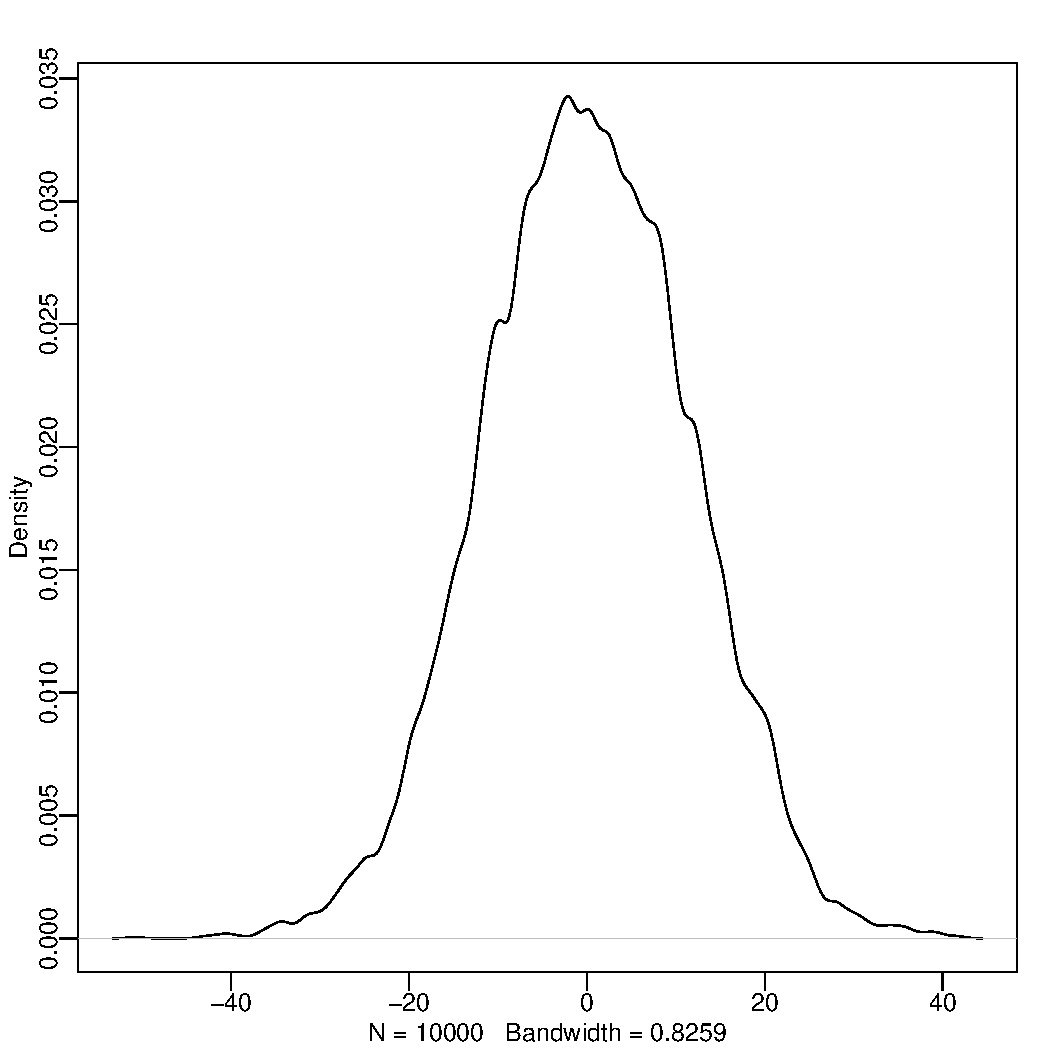
\includegraphics[width=\maxwidth]{figure/unnamed-chunk-2-1} 

\end{knitrout}

\begin{problem}{4M2}
\text{}\\
Translate the model just above into a \texit{map} formula.
\end{problem}

\begin{knitrout}
\definecolor{shadecolor}{rgb}{0.969, 0.969, 0.969}\color{fgcolor}\begin{kframe}
\begin{alltt}
\hlstd{flist} \hlkwb{<-} \hlkwd{alist}\hlstd{(}
  \hlstd{y} \hlopt{~} \hlkwd{dnorm}\hlstd{(mu, sigma),}
  \hlstd{mu} \hlopt{~} \hlkwd{dnorm}\hlstd{(}\hlnum{0}\hlstd{,} \hlnum{10}\hlstd{),}
  \hlstd{sigma} \hlopt{~} \hlkwd{dunif}\hlstd{(}\hlnum{0}\hlstd{,} \hlnum{10}\hlstd{)}
\hlstd{)}
\end{alltt}
\end{kframe}
\end{knitrout}

\begin{problem}{4M2}
\text{}\\
Translate the \texit{map} model formula below into a mathematical model definition.

\begin{knitrout}
\definecolor{shadecolor}{rgb}{0.969, 0.969, 0.969}\color{fgcolor}\begin{kframe}
\begin{alltt}
\hlstd{flist} \hlkwb{<-} \hlkwd{alist}\hlstd{(}
  \hlstd{y} \hlopt{~} \hlkwd{dnorm}\hlstd{(mu, sigma),}
  \hlstd{mu} \hlkwb{<-} \hlstd{a} \hlopt{+}\hlstd{b}\hlopt{*}\hlstd{x,}
  \hlstd{a} \hlopt{~} \hlkwd{dnorm}\hlstd{(}\hlnum{0}\hlstd{,} \hlnum{50}\hlstd{),}
  \hlstd{b} \hlopt{~} \hlkwd{dunif}\hlstd{(}\hlnum{0}\hlstd{,} \hlnum{10}\hlstd{),}
  \hlstd{sigma} \hlopt{~} \hlkwd{dunif}\hlstd{(}\hlnum{0}\hlstd{,} \hlnum{50}\hlstd{)}
\hlstd{)}
\end{alltt}
\end{kframe}
\end{knitrout}
\end{problem}

Model:
\begin{center}
y\textsubscript{i} $\sim$ Normal($\mu$, $\sigma$)\\
$\mu$ = $\alpha$ + $\beta$*x\textsubscript{i}\\
$\alpha$ $\sim$ Normal(0, 50)\\
$\beta$ $\sim$ Uniform(0, 10)\\
$\sigma$ $\sim$ Uniform(0, 50)
\end{center}


\end{document}
